\section{Полезные применения производной}
\epigraph{\textsf{in a dark place we find ourselves, and a little more knowledge lights our way.}}{\texttt{Yoda}}
Производная находит свое применение не просто в поиске точек роста и падения функции, а также в поиске ее минимального и максимального значения. 
На этом занятии мы разберемся как с помощью производной найти максимум потребляемой мощности в цепи, максимальную дальность полета мяча при броске и много чего другого в других науках, помимо физики.
\subsection{Экстремум}
Как мы уже поняли, если $z^{'} > 0$, то значение функции растет, если $z^{'} < 0$, то значение функции падает. Однако, если мы попадаем в $z^{'} = 0$, то это может говорить нам о том, что значение функции в данной точке находится на месте смена знака производной (если функция не постоянная, разумеется). То есть мы попали в локальный максимум или минимум этой функции.
\begin{theorem}[Ферма]
    Если функция $f(x)$ дифференцируема в точке $x_0$ и имеет в этой точке локальный \textbf{экстремум}, то $f^{'}(x_0) = 0$.
\end{theorem}
\begin{theorem}[достаточное условие экстремума]
    Пусть функция $z$ дифференцируема в окрестности точки $x_0$ - точки возможного экстремума. Если слева от этой точки ($x < x_0$) $z^{'} > 0\ (<0)$, а справа ($x > x_0$) $z^{'} < 0\ (>0)$, то в точка $x_0$ наблюдается \textbf{максимум/минимум}.
\end{theorem}
\begin{example}
    Известно, что сумма двух положительных чисел равна $12$. Какими должны быть эти числа, чтобы произведение их квадратов было максимальным?

    Надо решить систему уравнений
    \begin{equation*}
        \begin{cases}
            a + b = 12\\
            a^2b^2 \rightarrow \text{max}
        \end{cases} \Rightarrow
        f(a, b(a)) \equiv f(a) = a^2(12 - a)^2 = a^4 - 24a^3 + 144a^2
    \end{equation*}
    Наблюдаетя экстремум в точке $f^{'}(a) = 4a^3 -72a^2 + 288 a = 4a(a^2 - 18a + 72) =0 \Rightarrow a^2 - 18a + 72 = 0$. Решение $a_{1,2} = \frac{18 \pm 6}{2} = \{6, 12 \}$. А значит
    \begin{equation*}
        4a (a - 6)(a - 12) = 0 
    \end{equation*}
    Анализируя функцию производной, получим что максимум при значениях чисел $a = b = 6$.
\end{example}

\subsection{Производная x2, x3, x4 \dots}
Как вы можете заметить, функцию $f^{'}(x)$ можно дифференцировать далее. Мотивировать нас делать это можно тем, что в некоторых случаях это позволяет нам найти более точные значения экстремумов функции.
\begin{theorem}[достаточное условие экстремума через $2$-ю производную]
    Пусть функция $f$ непрерывна и дважды дифференцируема в точке $x_0$. Тогда при условии
    \begin{equation*}
        f^{'}(x_0) = 0, \quad f^{''}(x_0) < 0\ (>0)
    \end{equation*}
    в точке $x_0$ наблюдается локальный \textbf{максимум/минимум} функции $f$.
\end{theorem}
Если же функция дифференцируема большее число раз, то мы можем использовать $n$-ю производную для нахождения экстремума функции.
\begin{theorem}[достаточное условие экстремума через $n$-ю производную]
    Пусть функция $f$ непрерывна и $n$-кратно дифференцируема в точке $x_0$. Тогда при условии
    \begin{equation*}
        f^{'}(x_0) = 0, \quad f^{''}(x_0) = 0, \quad \dots, \quad f^{(n-1)}(x_0) = 0, \quad f^{(n)}(x_0) < 0\ (>0)
    \end{equation*}
    в точке $x_0$ наблюдается локальный \textbf{максимум/минимум} функции $f$.
\end{theorem}
\begin{prac}
    Решить предыдущую задачу через вторую производную.
\end{prac}

\begin{example}
    Найти $n$-ю производную функции $y = \frac{x^2 + 1}{x^2 - 1}$.

    Так как $y = 1 + \frac{1}{x - 1} - \frac{1}{x+1}$, то можно просто поисследовать взятие производной каждого слагаемого
    \begin{eqnarray*}
        \bigl(\frac{1}{x-1}\bigr)^{(n)} &= (-1)\bigl(\frac{1}{x - 1}\bigr)^{(n-1)} = (-1)^2 \cdot 2\bigl(\frac{1}{x - 1}\bigr)^{(n-2)} = \dots = (-1)^n \cdot n! \cdot (x - 1)^{-n}\\
        \bigl(\frac{1}{x+1}\bigr)^{(n)} &= (-1)\bigl(\frac{1}{x + 1}\bigr)^{(n-1)} = (-1)^2 \cdot 2\bigl(\frac{1}{x + 1}\bigr)^{(n-2)} = \dots = (-1)^n \cdot n! \cdot (x + 1)^{-n}
    \end{eqnarray*}
    тогда получим ответ
    \begin{equation*}
        y^{(n)} = (-1)^n\ n!\ \Bigl(\frac{1}{(x - 1)^n} + \frac{1}{(x + 1)^n}\Bigr)
    \end{equation*}
\end{example}

\subsection{Разговор о минимумах и максимумах}
Теперь мы набили руку в взятии производных, поиске экстремумов и даже в нахождении $n$-й производной функции. Теперь приступим к самому интересному - поиску минимумов и максимумов в физике. Но перед физиков разомнемся на геометрии.
\begin{example}[Задача Евклида]
    В данный треугольник \textit{ABC} вписать параллелограмм \textit{ADEF} (\textit{EF} $\Vert$ \textit{AB}, \textit{DE} $\Vert$ \textit{AC}) наибольшей площади.

    \begin{figure}[h!]
        \centering
        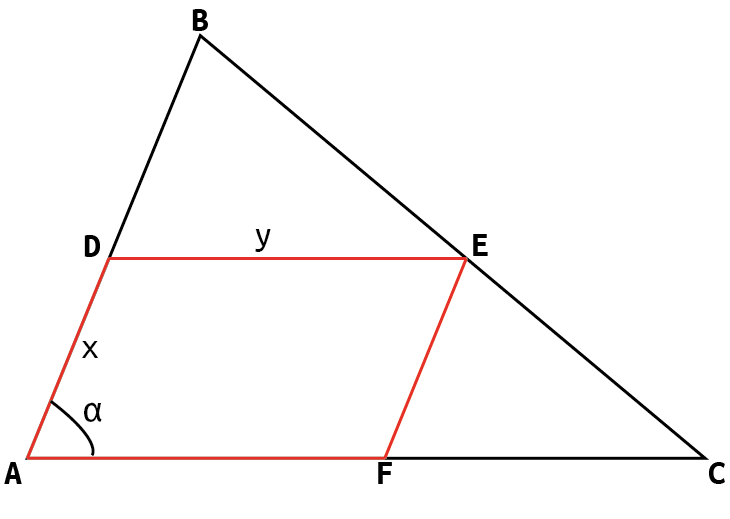
\includegraphics[scale=0.5]{pics/geom_evklid.png}
        \caption{Задача Евклида}
    \end{figure}

    Пусть $x = AD,\ y = AF, \alpha = \angle DAF$. Выпишем площадь параллелограмма: $S_{ADEF} = \frac{1}{2} xy \sin \alpha$. Площадь $\Delta ABC$ можно выразить несколькими способами
    \begin{equation*}
        \frac{1}{2} AB\ AC\ \sin \alpha = S_{ABC} = S_{ADEF} + \frac{1}{2} (AB - x) y \sin \alpha + \frac{1}{2} (AC - y) x \sin \alpha
    \end{equation*}
    Тогда получим задачу
    \begin{equation*}
        \begin{cases}
            AB \cdot y + AC \cdot x = AB \cdot AC\\
            xy \rightarrow \text{max}
        \end{cases}
    \end{equation*}
    Нужно найти максимум функции $f(x) = -x^2 \frac{AC}{AB} + AC \cdot x$ (\textbf{узнали задачу ?}). Решаем
    \begin{equation*}
        f^{'}(x) = -2x \frac{AC}{AB} + AC = 0 \Rightarrow x = \frac{AB}{2},\ y = \frac{AC}{2}
    \end{equation*}
    Таким образом мы решили задачу Евклида и нашли, что параллелограмм наибольшей площади вписан в треугольник, если его стороны равны половине сторон треугольника.
\end{example}
Finally, физика!
\begin{example}
    Тело массой $m$, находящееся на горизонтальной поверхности, испытывает действие постоянной по модулю силы $F$. Угол $\alpha$ между вектором силы и горизонтом можно изменять. Определить максимально возможное ускорение тела. Коэффициент трения между телом и поверхностью равен $\mu$.

    \begin{figure}[h!]
        \centering
        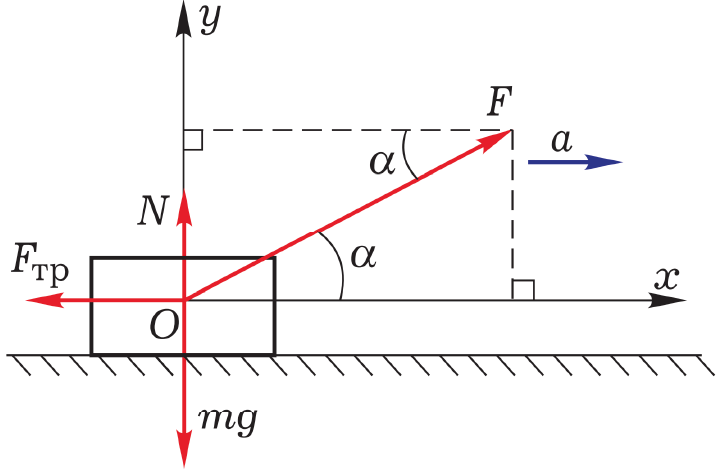
\includegraphics[scale=0.7]{pics/phys_force_extr.png}
        \caption{Рисунок к задачке}
    \end{figure}

    Второй закон Ньютона в проекции по осям
    \begin{eqnarray*}
        OX: && F \cos \alpha - \mu N = m a\\
        OY: && F \sin \alpha  +N - mg = 0
    \end{eqnarray*}
    Ускорение $a = \frac{F}{m} \bigl(\cos \alpha + \mu \sin \alpha \bigr) - \mu g$. Приравняем к нулю производную по углу
    \begin{equation*}
        \frac{da}{d\alpha} = \frac{F}{m} \bigl(-\sin \alpha + \mu \cos \alpha \bigr) = 0 \Rightarrow \tan \alpha_{0} = \mu
    \end{equation*}
    А значит 
    \begin{equation*}
        a_{\text{max}} = \frac{F}{m} \sqrt{1 + \mu^2} - \mu g
    \end{equation*}
    \textbf{почему это максимум?}
\end{example}
\subsection{Ряд Тейлора, детка}
Зачастую значение функции приходится считать приближенно в какой-либо точке $x_0$ в рамках заданных условий задачи. Например, в задачах геометрической оптики используют приближение малых углов отклонения. Исследовать поведение функции в окрестности точки $x_0$ можно с помощью ряда Тейлора.
\begin{definition}
    \textbf{Ряд Тейлора} $n$ раз непрерывно-дифференцируемой функции $f(x)$ в точке $x_0$ - это ряд вида
    \begin{equation*}
        f(x) = \sum_{k = 0}^{n}\frac{f^{(k)}(x_0)}{k!} (x - x_0)^k + R_{n+1}(x),
    \end{equation*}
    где $R_{n+1}(x)$ - остаточный член, который стремится к нулю при $x \to x_0$.
\end{definition}

Распишим основные функции в ряд Тейлора в окрестности точки $x_0 = 0$. Такое разложение вблизи $0$ \textbf{рядом Маклорена}:
\begin{itemize}
    \item $e^{x} = \sum_{k = 0}^{\infty} \frac{x^k}{k!} \approx 1 + x$
    \item $\sin x = \sum_{k = 0}^{\infty} \frac{x^{2k + 1}}{(2k + 1)!} \approx x - \frac{x^3}{3}$
    \item $\cos x = \sum_{k = 0}^{\infty} \frac{(-1)^k x^{2k}}{(2k)!} \approx 1 - \frac{x^2}{2}$
\end{itemize}

\begin{example}[Формула Эйлера]
    Докажем одну из самых красивых формул математики
    \begin{equation*}
        e^{ix} = \cos x + i \sin x
    \end{equation*}
    Разложим экспоненту в ряд Маклорена
    \begin{multline*}
        e^{ix} = \sum_{k = 0}^{\infty} \frac{(ix)^k}{k!} = \{i^2 = -1, i^3 = -i, \dots \}= \sum_{k = 0}^{\infty} \frac{x^{2k}}{(2k)!} + i \sum_{k = 0}^{\infty} \frac{x^{2k + 1}}{(2k + 1)!} = \\
        = \cos x + i \sin x
    \end{multline*}
    Эта формула будет встречаться во множестве физических задач, особенно в квантовой механике, где она используется для описания волновых функций частиц.
\end{example}